\documentclass[10pt]{article}  

\usepackage[catalan]{babel}
\usepackage[utf8]{inputenc}  
\usepackage{graphicx}
\usepackage{color}
\usepackage{float}
\usepackage{caption}

\usepackage{anysize}
\marginsize{2cm}{2cm}{2cm}{2cm} % Izquierda, derecha, arriba, abajo

\usepackage[colorlinks=true,plainpages=true,citecolor=blue,linkcolor=blue]{hyperref}

% Para agregar encabezado y pie de página
\usepackage{fancyhdr} 
\pagestyle{fancy}
\fancyhf{}
\fancyhead[L]{\footnotesize XARXES I COMUNICACIONS} %encabezado izquierda
\fancyhead[R]{\footnotesize EPS-UdL}   % dereecha
\fancyfoot[R]{\footnotesize Pràctica 1}  % Pie derecha
\fancyfoot[L]{\footnotesize Grau en Enginyeria Informàtica}  %izquierda
\renewcommand{\footrulewidth}{0.4pt}

%%%%%%%% TERMINA PREÁMBULO %%%%%%%%%%%%

\begin{document}

%%%%%%%%%%%%%%%%%%%%%%%%%%%%%%%%%% PORTADA %%%%%%%%%%%%%%%%%%%%%%%%%%%%%%%%%%%%%%%%%%%%
                                                                                    %%%
\begin{center}                                                                      %%%
\newcommand{\HRule}{\rule{\linewidth}{0.5mm}}                                   %%%\left
                                                                                    %%%
\begin{minipage}{0.48\textwidth} \begin{flushleft}

\includegraphics[scale = 0.23]{Images/logo_udl.jpg}
\end{flushleft}\end{minipage}
\begin{minipage}{0.48\textwidth} \begin{flushright}

\includegraphics[scale = 0.25]{Images/logo_eps.jpg}
\end{flushright}\end{minipage}

                                                                                    %%%
\vspace*{-1.5cm}                                %%%
                                                                                    %%% 
\textsc{\huge ESCOLA POLIT\` ECNICA \\ \vspace{5px}SUPERIOR}\\[1.5cm] 

\textsc{\LARGE XARXES I COMUNICACIONS}\\[1.5cm]                                                   %%%

\begin{minipage}{0.9\textwidth} 
\begin{center}                                                                                  %%%
\textsc{\LARGE PR\`ACTICA 1}
\end{center}
\end{minipage}\\[0.5cm]
%%%
                                                                                    %%%
            \vspace*{1cm}                                                                       %%%
                                                                                    %%%
\HRule \\[0.4cm]                                                                    %%%
{ \huge \bfseries RIP, OSPF \& BGP}\\[0.4cm]  %%%
                                                                                    %%%
\HRule \\[1.5cm]                                                                    %%%
                                                                                %%%
                                                                                    %%%
\begin{minipage}{0.46\textwidth}                                                    %%%
\begin{flushleft} \large                                                            %%%
\emph{Students:}\\   
Nil Agut Marín\\
Jaume Giralt Barbé
%%%
            %\vspace*{2cm}  
                                                                %%%
                                                                %%%
\end{flushleft}                                                                     %%%
\end{minipage}      
                                                                %%%
\begin{minipage}{0.52\textwidth}        
\vspace{-0.6cm}                                         %%%
\begin{flushright} \large                                                           %%%
\emph{Professor:} \\                                                                 %%%
Fernández Camon, Cèsar                                                    %%%
\end{flushright}                                                                    %%%
\end{minipage}  
\vspace*{1cm}
%\begin{flushleft}
    

\begin{center}                                                                                  
{\large \today}                                                                 %%%
            \end{center}                                                                        
\end{center}                                                                        
                                                                                    
\newpage                                                                        
%%%%%%%%%%%%%%%%%%%% TERMINA PORTADA %%%%%%%%%%%%%%%%%%%%%%%%%%%%%%%%

\tableofcontents
\listoffigures 

\newpage

\section{Objectius}
L'objectiu principal d'aquesta pràctica és implementar els protocols apresos a classe per a 

\section{Topologia de la xarxa}
\begin{figure}[H]
\begin{center}
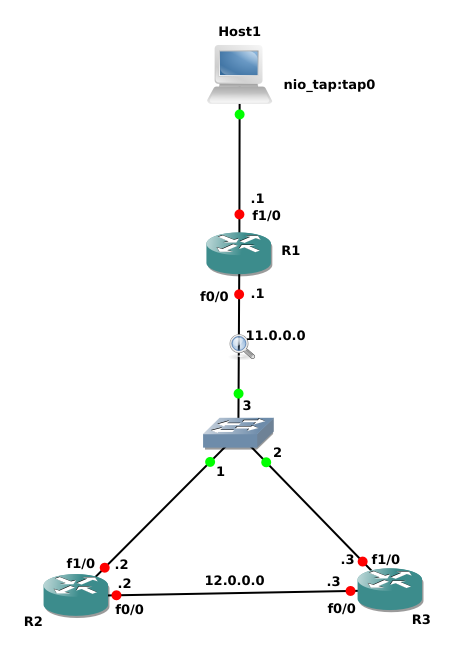
\includegraphics[scale=0.5]{Images/screenshot.png}
\caption{Topologia de la xarxa a efectuar l'exercici}
\end{center}
\end{figure}
Per a la realització de aquest exercici utilitzarem encaminadors \textbf{Cisco c7200} 
\subsection{Encaminador 1}
sssss
\section{Valors per defecte del encaminador}
\textbf{Quins són els valors per defecte per els paquets \textit{update, invalid} i \textit{flush} ?\\Utilitza les comandes del encaminador i el programari Wireshark}
\\\\
Per a comprovar el temps per defecte


\end{document}
              
